\documentclass[11pt]{book}

\usepackage[utf8]{inputenc}
\usepackage{t1enc}
\usepackage[magyar]{babel}
\usepackage{lipsum}
\usepackage{xcolor}
\usepackage{geometry}
\usepackage{fancyhdr}
\usepackage{graphicx}
\usepackage{caption}
\usepackage{subcaption}
\usepackage{wrapfig}
\usepackage{amsfonts}
\usepackage{amsmath}
\usepackage{algpseudocode}
\usepackage{forloop}

\geometry{headheight=14pt}
\pagestyle{fancy}
\fancyhead[LE,RO]{}
\fancyhead[RE]{Fejezet \thechapter}
\fancyhead[LO]{Section \thesection}
\fancyfoot[C]{}
\fancyfoot[RE,LO]{\thepage}

\title{Zárthelyi Dolgozat\\ {\small A Csoport}}
\author{Orosz Péter - WO02D7}

\newtheorem{definicio}{Definíció}
\newtheorem{tetel}{Tétel}

\newenvironment{my_verse}[2]{
	\begin{center}
		\textbf{#2}\\
		\textit{#1}
	\end{center}
}

\begin{document}
	\maketitle
	\newpage
	\chapter{1. Feladat}
		\section{Első Section}
			\lipsum
		\section{Második Section}
			\lipsum
			
	\chapter{2. Feladat}
		\lipsum[1-4]
		\begin{wrapfigure}{r}{0.5\textwidth}
			\centering
			\caption{Színes és Szépia Képek}
			\begin{subfigure}{5cm}
				\centering
				\caption{Színes Kép}
				\scalebox{0.5}[1.0]{
\includegraphics[height=4cm]{szines.jpg}}
			\end{subfigure}\\
			\begin{subfigure}{5cm}
				\centering
				\caption{Szépia Kép}
				\framebox{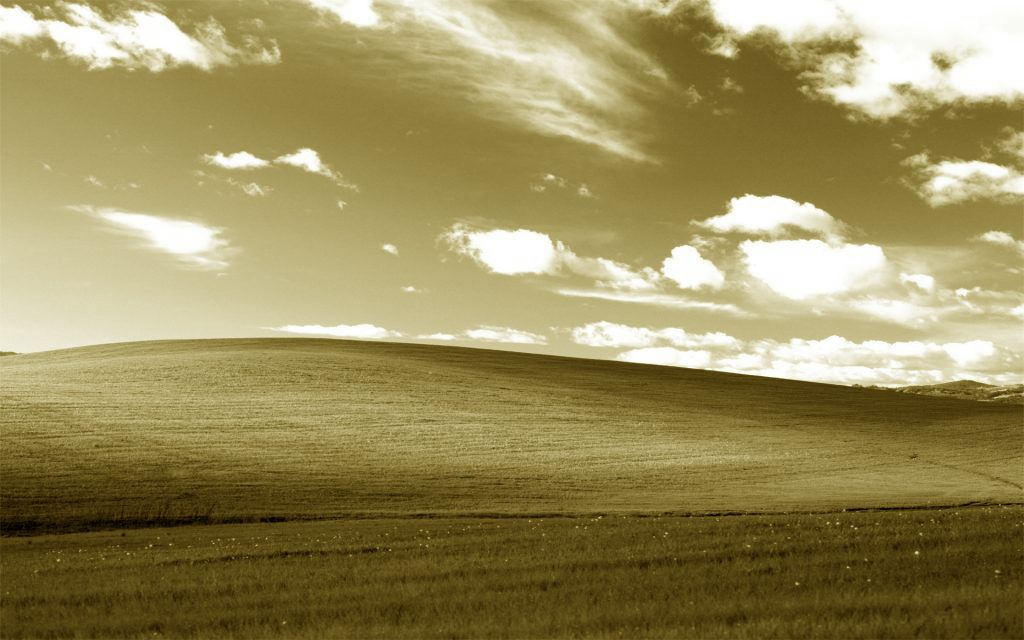
\includegraphics[height=4cm]{szepia.jpg}}
			\end{subfigure}
		\end{wrapfigure}
		\lipsum
	
	\chapter{3. Feladat}
		\begin{definicio}[Sajátérték]
			Legyen $A \in \mathbb{R}^{n \times n}$ négyzetes mátrix. Azt mondjuk, hogy $\lambda \in \mathbb{C}$ sajátértéke és $v \in \mathbb{C}^n$ a $\lambda$ sajátértékéhez tartozó (jobb oldali) sajátvektora $A$-nak, ha 
			\begin{gather}
				Av=\lambda v.
			\end{gather}
		\end{definicio}
		
		\begin{definicio}{Karakterisztikus Polinom}
			Jelölje $E = \mathbb{R}^{n\times n}$ az egységmátrixot.\\
			Az $A$ ún. \textit{karakterisztikus polinomja}
			\begin{gather}
                \varphi(\lambda) := det(A\textcolor{red}{-\lambda E})=
                \left| 
                	\begin{matrix}
                        a_{11}\textcolor{red}{-\lambda} & a_{12} & \cdots & a_{1n}\\
                   		a_{21} & a_{22}\textcolor{red}{-\lambda} & \cdots & a_{2n}\\
                       	\vdots & \vdots & \ddots & \vdots\\
                   		a_{n1} & a_{n2} & \cdots & a_{nn}\textcolor{red}{-\lambda}
                	\end{matrix} 
             	\right|,
            \end{gather}
             egy $n$-edfokú polinom $\lambda$-ban. 
		\end{definicio}
		
		\begin{tetel}{Sajátérték meghatározása}
			Az $A \in \mathbb{R}^{n \times n}$ mátrix sajátértékei az ún. \textit{karakterisztikus egyenlet}
			\begin{gather}
				\varphi(\lambda) = 0
			\end{gather}
			megoldásai. Mivel a $\varphi(\lambda)$ \textit{karakterisztikus polinom} egy $n$-edfokú polinom $\lambda$-ban, ezért a komplex számokon (multiplicitással együtt) $n$ megoldás van.
		\end{tetel}
		
		\chapter{4. Feladat}
		
		\chapter{5. Feladat}
			\begin{my_verse}{my author}{my title}
				
				Vers Első Versszak Első sor\\
				Vers Első Versszak Második sor\\
				Vers Első Versszak Harmadik sor\\
				Vers Első Versszak Negyedik sor\\
				
				Vers Második Versszak Első sor\\
				Vers Második Versszak Második sor\\
				Vers Második Versszak Harmadik sor\\
				Vers Második Versszak Negyedik sor\\
			\end{my_verse}
			
		\chapter{+1. Feladat}
		
		\newcounter{x}
		\newcounter{even}{0}
		\forloop{x}{1}{\value{x} < 61}{ 
			\ifnum \value{even}=1
				\textcolor{red}{\arabic{x}}
				\setcounter{even}{0}
			\else
				\arabic{x}
				\setcounter{even}{1}
			\fi
    		                 
}
\end{document}